%! Author = borisdeletic
%! Date = 03/05/2023

% Preamble
\documentclass[11pt]{article}
\usepackage{algpseudocode}


% Document
\begin{document}

\section{Constrained Hamiltonian Monte Carlo}\label{sec:chmc}
    Consider the constrained prior distribution subject to the hard likelihood constraint
    \begin{equation}\label{eq:constrained_prior}
        \tilde{\pi}(\theta) = \begin{cases}
                                  \pi(\theta), & \mathcal{L}(\theta) > \mathcal{L}_0 \\
                                  0, & \text{otherwise}
                              \end{cases}
    \end{equation}
    Hamiltonian Monte Carlo can be modified to sample from a constrained distribution, making it a viable
    technique for generating new live points in nested sampling.
    As described conceptually by Skilling~\cite{GMC} \& Betancourt~\cite{Betancourt_NS_CHMC}, reflecting
    off the iso-likelihood contours ensures that proposed samples are within the constrained distribution.
    When the next position $\mathbf{x}$ in the trajectory would be below the likelihood constraint, we reflect the
    momentum off the boundary with normal $n$
    \begin{equation}\label{eq:reflection}
    \begin{aligned}
        \mathbf{n} &= - \nabla \log{\mathcal{L}}, \\
        \mathbf{n_R} &= M^{-1} \mathbf{n}, \\
        \mathbf{p'} &= \mathbf{p} - 2 \frac{ \mathbf{p} \cdot \mathbf{n_R} }{\mathbf{n} \cdot \mathbf{n_R}}. \mathbf{n}
    \end{aligned}
    \end{equation}

    \begin{figure}[t!]
        \center
        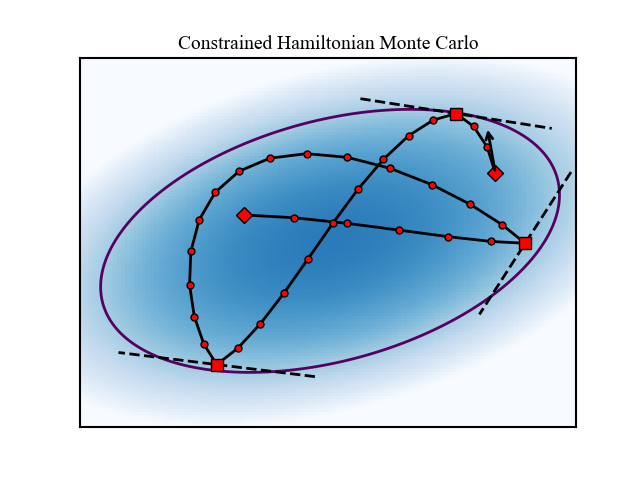
\includegraphics[width=\linewidth]{../figures/ConstrainedHMC}
        \caption{
        Hamiltonian Monte Carlo modified to reflect off iso-likelihood boundary $\mathcal{L}_0$.
        Initial point with randomly sampled
        momentum (diamond with arrow) moving through prior distribution, $\tilde{\pi}(\theta)$, shown in blue. Finite step size $\epsilon$,
        shows discretisation of integrator with intermediate points (circles). Points which reflect off
        boundary (squares) do not fall exactly on the boundary due to discretization. After a fixed number of
        integration steps $L$, we propose a new sample from the constrained distribtion (diamond).
        }\label{fig:constrainedhmc}
    \end{figure}

    At iteration $i$ of nested sampling, the point with the lowest likelihood $\mathcal{L}_i$ is deleted and used to
    seed the generation of the next sample.
    Implementing this algorithm in practice poses new challenges with discretization, clustering, and parameter adaption.
    We propose a novel set of additional algorithms which are essential for a working implementation of
    Constrained HMC (CHMC).

\subsection{Epsilon Halving}\label{subsec:epsilon_halving}
    When performing reflections with a finite step size $\epsilon$, there is no guarantee that after a reflection,
    the next point will be within the constrained boundary.
    While this scenario is uncommon for smooth boundaries, over many iterations it is likely that at one time,
    no valid reflection will be found, causing the algorithm to crash.

    \begin{figure}[t!]
        \center
        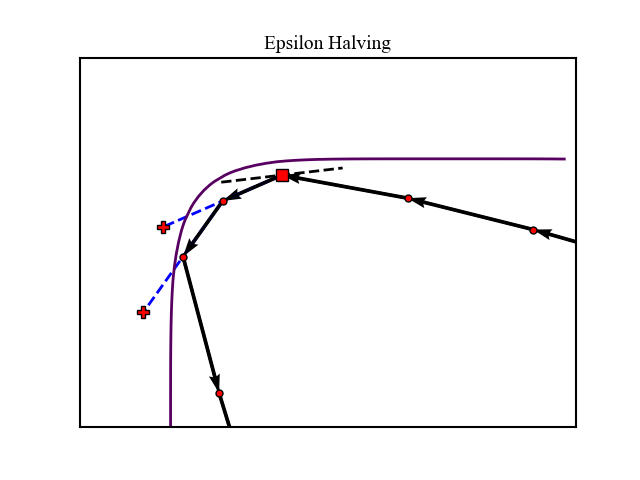
\includegraphics[width=\linewidth]{../figures/EpsilonHalving}
        \caption{
        For sharply curved boundaries, it is possible for the reflected points (plus) to also lie outside the boundary
        constraint, leaving no valid reflections.
        In order for the algorithm to continue, a temporary step size is used to calculate the next position only.
        We iterate $\epsilon' = \epsilon / 2$ until the next point lies within the constraint.
        After a valid point is found, we return back to integrating with $\epsilon_0$.
        }\label{fig:epsilon_halving}
    \end{figure}

    We propose a new reflection scheme which guarantees that a valid reflection will always be found, allowing the
    algorithm to continue.
    After a reflection, the next point is checked to see if it lies outside the boundary.
    If so, a temporary step size $\epsilon' = \epsilon / 2$ is used to re-integrate the position of the next point.
    Epsilon is repeatedly halved until a valid next point is found.
    This is guaranteed to find a valid reflection as the limit $\epsilon' -> 0$ performs a continous reflection.
    The algorithm then continues with the original $\epsilon_0$. \\

    \begin{algorithm}
        \caption{Epsilon Halving}
        \label{alg:epsilon_halving}
        \begin{algorithmic}
            \STATE \COMMENT{Momentum reflection}
            \STATE $\mathbf{p} \gets \mathbf{p} - 2 \left(\mathbf{p} \cdot \hat{ \mathbf{n} } \right) \hat{ \mathbf{n} }$
            \STATE
            \STATE $ \mathbf{x_{new}} \gets \mathbf{x} + \epsilon_0 \mathbf{p}$
            \STATE $ \epsilon' \gets \epsilon_0$
            \STATE
            \WHILE{ $\mathcal{L}(\mathbf{x_{new}}) < \mathcal{L}_0$ }
                \STATE $\epsilon' \gets \epsilon' / 2$
                \STATE $ \mathbf{x_{new}} \gets \mathbf{x} + \epsilon' \mathbf{p}$
            \ENDWHILE
            \STATE
            \STATE $\mathbf{x} \gets \mathbf{x_{new}}$
        \end{algorithmic}
    \end{algorithm}


\subsection{Ergodicity}\label{subsec:ergodicity}
    Ergodicity and detailed balance are well known to be requirements of any MCMC algorithm~\cite{Metropolis_OG}.
    However, in practice no algorithm is truly ergodic due to imperfections in computation such as floating-point
    errors and the cyclic nature of pseudo-random number generators.
    The question then becomes whether the algorithm is \emph{sufficiently ergodic}.
    It is clear the process introduced by epsilon halving is not ergodic, therefore it is essential we ask
    whether our algorithm will maintain sufficient ergodicity.

    Adaptive techniques in MCMC methods have been shown to still converge to the required
    distribution~\cite{MCMC_Ergodicity}.
    Therefore, we argue that so long as our non-ergodic techniques are used infrequently, CHMC will be sufficiently
    ergodic to pass all statistical tests.

\subsection{Clustering}\label{subsec:clustering}

    Multi-modal posteriors pose a challenging problem for many MCMC sampling algorithms with topological freezing
    causing complications~\cite{mangoubi2018_HMC_Multimodal}.
    In theory, nested sampling solves multi-modal distributions without difficulty, hence its appeal as a tool for
    Bayesian inference.
    However, in practice it is important to carefully consider the sampling methods to ensure that they do not
    cause a systematic bias.
    For instance, if there are not enough live points, it is possible for modes to 'die out' and be missed by nested
    sampling.
    This necessitates for special measures in order to identify clusters of live points and treat them separately,
    as explored by \textsc{PolyChord} which uses a k-means algorithm for this purpose~\cite{Handley_polychord}.

    We illustrate how CHMC naturally solves clustering.
    In nested sampling of multimodal distributions, once the likelihood constraint is raised to the point where the
    contour splits into the two modes, all live points in separate modes evolve completely independently of each other.

    \begin{figure}[t!]
        \center
        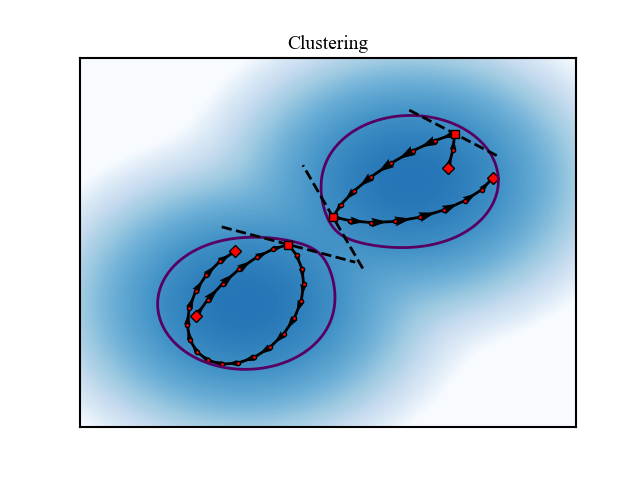
\includegraphics[width=\linewidth]{../figures/Clustering}
        \caption{
        Clustering in multi-modal distributions. When the iso-likelihood contour splits into
        two isolated modes, new samples generated are prevented from mixing with each other.
        The position $\mathbf{\theta}$ is restricted to stay within the posterior region contained by the boundary,
        as all intermediate points have no mechanism to cross into the other mode.
        }\label{fig:clustering}
    \end{figure}

\subsection{Topological Traps}\label{subsec:topological_trap}
    The natural clustering advantage of CHMC also brings rise a susceptibility to topological traps.
    Any live points in a local maxima will be forced to stay there, becoming further and further compressed until there
    is no more space new samples to be generated.

    We propose a new mechanism for sampling through topological traps.
    Define the \emph{reflection rate} for live point i as
    \begin{equation}\label{eq:reflect_rate}
        \mathcal{R}_i = \frac{r_i}{L},
    \end{equation}
    where $r_i$ is the number of reflections in the CHMC evolution.
    The motivation is that as we repeatedly resample points in an ever more constrained local maximum,
    $\mathcal{R}$ will approach 1 for these live points.

    \begin{algorithm}
        \caption{Nested sampling through topological traps using reflection rate}
        \label{alg:reflection_rate}
        \begin{algorithmic}
            \VARIABLES
            \STATE $\mathcal{R}_0$, Reflection rate threshold
            \STATE $\theta_i$, Parameters for live point with lowest likelihood at iteration i
            \STATE $\theta_r$, Parameters for a random live point
            \ENDVARIABLES
            \STATE
            \IF{ $\mathcal{R}(\theta_i) < \mathcal{R}_0$ }
            \STATE $\theta_{i+1} \gets$ \text{CHMC}($\theta_i$)
            \ELSE
            \STATE $\theta_{i+1} \gets$ \text{CHMC}($\theta_r$)
            \ENDIF
        \end{algorithmic}
    \end{algorithm}

    When a dead point has a reflection rate above some threshold, $\mathcal{R}_0$, we use a random live point as
    the seed for the next iteration, instead of the dead point.
    This ensures that if at least one live point is in the global maximum, eventually all the new live points will move
    into this mode where there is more `space`.

    Show tests.
\end{document}